\documentclass[
  bibliography=totoc,     % Literatur im Inhaltsverzeichnis
  captions=tableheading,  % Tabellenüberschriften
  titlepage=firstiscover, % Titelseite ist Deckblatt
]{scrartcl}

% Paket float verbessern
\usepackage{scrhack}

% Warnung, falls nochmal kompiliert werden muss
\usepackage[aux]{rerunfilecheck}

% unverzichtbare Mathe-Befehle
\usepackage{amsmath}
% viele Mathe-Symbole
\usepackage{amssymb}
% Erweiterungen für amsmath
\usepackage{mathtools}

% Fonteinstellungen
\usepackage{fontspec}
% Latin Modern Fonts werden automatisch geladen
% Alternativ:
%\setromanfont{Libertinus Serif}
%\setsansfont{Libertinus Sans}
%\setmonofont{Libertinus Mono}
\recalctypearea % Wenn man andere Schriftarten gesetzt hat,
% sollte man das Seiten-Layout neu berechnen lassen

% deutsche Spracheinstellungen
\usepackage{polyglossia}
\setmainlanguage{german}


\usepackage[
  math-style=ISO,    % ┐
  bold-style=ISO,    % │
  sans-style=italic, % │ ISO-Standard folgen
  nabla=upright,     % │
  partial=upright,   % ┘
  warnings-off={           % ┐
    mathtools-colon,       % │ unnötige Warnungen ausschalten
    mathtools-overbracket, % │
},                       % ┘
]{unicode-math}

% traditionelle Fonts für Mathematik
\setmathfont{Latin Modern Math}
% Alternativ:
%\setmathfont{Libertinus Math}

\setmathfont{XITS Math}[range={scr, bfscr}]
\setmathfont{XITS Math}[range={cal, bfcal}, StylisticSet=1]

% Zahlen und Einheiten
\usepackage[
locale=DE,                   % deutsche Einstellungen
separate-uncertainty=true,   % immer Fehler mit \pm
per-mode=symbol-or-fraction, % / in inline math, fraction in display math
]{siunitx}

% chemische Formeln
\usepackage[
version=4,
math-greek=default, % ┐ mit unicode-math zusammenarbeiten
text-greek=default, % ┘
]{mhchem}

% richtige Anführungszeichen
\usepackage[autostyle]{csquotes}

% schöne Brüche im Text
\usepackage{xfrac}

% Standardplatzierung für Floats einstellen
\usepackage{float}
\floatplacement{figure}{htbp}
\floatplacement{table}{htbp}

% Floats innerhalb einer Section halten
\usepackage[
section, % Floats innerhalb der Section halten
below,   % unterhalb der Section aber auf der selben Seite ist ok
]{placeins}

% Seite drehen für breite Tabellen: landscape Umgebung
\usepackage{pdflscape}

% Captions schöner machen.
\usepackage[
  labelfont=bf,        % Tabelle x: Abbildung y: ist jetzt fett
  font=small,          % Schrift etwas kleiner als Dokument
  width=0.9\textwidth, % maximale Breite einer Caption schmaler
]{caption}
% subfigure, subtable, subref
\usepackage{subcaption}

% Grafiken können eingebunden werden
\usepackage{graphicx}
% größere Variation von Dateinamen möglich
\usepackage{grffile}

% schöne Tabellen
\usepackage{booktabs}

% Verbesserungen am Schriftbild
\usepackage{microtype}

% Literaturverzeichnis
\usepackage[style=alphabetic,]{biblatex}
% Quellendatenbank
\addbibresource{lit.bib}

% Hyperlinks im Dokument
\usepackage[
  unicode,        % Unicode in PDF-Attributen erlauben
  pdfusetitle,    % Titel, Autoren und Datum als PDF-Attribute
  pdfcreator={},  % ┐ PDF-Attribute säubern
  pdfproducer={}, % ┘
]{hyperref}
% erweiterte Bookmarks im PDF
\usepackage{bookmark}

% Trennung von Wörtern mit Strichen
\usepackage[shortcuts]{extdash}

\title{V408: Geometrische Optik}
\author{
  Simon Schulte
  \texorpdfstring{
    \\
    \href{mailto:simon.schulte@udo.edu}{simon.schulte@udo.edu}
  }{}
  \texorpdfstring{\and}{, }
  Tim Sedlaczek
  \texorpdfstring{
    \\
    \href{mailto:tim.sedlaczek@udo.edu}{tim.sedlaczek@udo.edu}
  }{}
}
\publishers{TU Dortmund – Fakultät Physik}

\date{Durchführung: 02.05.2017\\
      Abgabe: 09.05.2017}


\begin{document}

\maketitle
\thispagestyle{empty}
\tableofcontents
\newpage
\setcounter{page}{1}
\section{Zielsetzung}
\label{sec:zielsetzung}
In diesem Versuch sollen die Brennweiten von Linsen und Linsensystemen bestimmt
werden.
\section{Theorie}
\label{sec:theorie}
Die Meisten Linsen bestehen aus Glas. In diesem Versuch wird auch eine mit Wasser
gefüllte Linse verwendet. Entscheidend ist, dass diese Linsen aus einem Material
sind, welches optisch dichter ist als die Umgebung. So wird das Licht an ihren
Oberflächen gebrochen. Dabei ist zwischen zwei Arten von Linsen zu unterscheiden.
Den Sammellinsen, welche wegen ihrer Form das Licht bündeln und eine positive
Brennweite besitzen, und den Streuungslinsen, welche Gegenteiliges bewirken und
eine negative Brennweite besitzen. Bei Sammellinsen entsteht dabei ein reelles
Bild, während bei Streuungslinsen ein virtuelles Bild entsteht (d.h., dass die
Bildweite negativ ist).

\noindent
Wie in Abbildung \ref{fig:V4081} zu sehen ist werden zur Bildkonstruktion
drei Strahlen verwendet, welche sich dadurch auszeichnen, dass sie durch einen
der Brennpunkte oder durch den Mittelpunkt der Linse verlaufen.
Mithilfe der Strahlensätze ergibt sich das so genannte Abbildungsgesetz
\begin{equation}
  V = \frac{B}{G} = \frac{b}{g}.
  \label{eqn:abbildung}
\end{equation}\\
Dabei wird $V$ als Abbildungsmaßstab bezeichnet. $B$ ist die Bildgröße, $G$ die
Gegenstandsgröße, $b$ die Bildweite und $g$ die Gegenstandsweite.
Zusätzlich ergibt sich daraus die Linsengleichung
\begin{equation}
  \frac{1}{f} = \frac{1}{g} + \frac{1}{b}.
  \label{eqn:linsen}
\end{equation}\\
Für dünne Linsen wird vereinfachend angenommen, dass das Licht an der Mittelebene
gebrochen wird. Für dickere Linsen und Linsensysteme gilt dies nicht mehr.
Als Vereinfachung ergeben sich dann zwei Hauptebenen $H$ und $H'$,
für die Bild- und für die Gegenstandsweite, für die die Linsengleichung dann
erfüllt ist.

\noindent
Bei Linsen und Linsensystemen entstehen im Allgemeinen zwei Abbildungsfehler.
Aufgrund der sphärischen Form besitzen Linsen für achsenferne Strahlen
unterschiedliche Brennpunkte, die von der eigentlichen Brennweite abweichen.
Dem kann durch einen speziellen Schliff oder durch eine Irisblende entgegengewirkt
werden.

\noindent
Zudem zeigt sich für verschiedene Wellenlängen im Licht ein unterschiedliches
Brechungsverhalten, weshalb die Brennweite der Linse für verschiedene Farben
variiert.
\clearpage
\section{Durchführung}
\subsection{Versuchsaufbau}
Der Versuchsaufbau besteht aus einer Halogenlampe, einem Gegenstand $G$ (eine
Blende aus L-förmig angeordnetten Kreisblenden), verschiedenen Linsen, zwei
Farbfiltern und einem Schirm, auf den das Bild $B$ projiziert wird.

\noindent
In den Abbildungen \ref{fig:V4081} bis \ref{fig:V4083} sind die schematischen
Aufbauten bzw. die Bildkonstruktionen für die verschiedenen Messungen dargestellt.
\begin{figure}[htb]
  \centering
  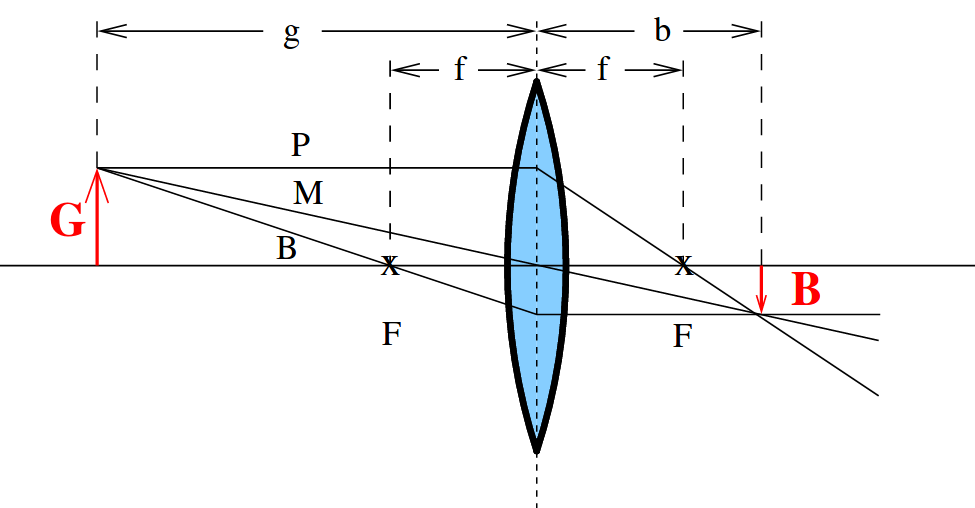
\includegraphics[width=0.8\textwidth]{V4081.png}
  \caption{Aufbau für den ersten Versuchsteil \cite{anleitung}.}
  \label{fig:V4081}
\end{figure}
\begin{figure}[htb]
  \centering
  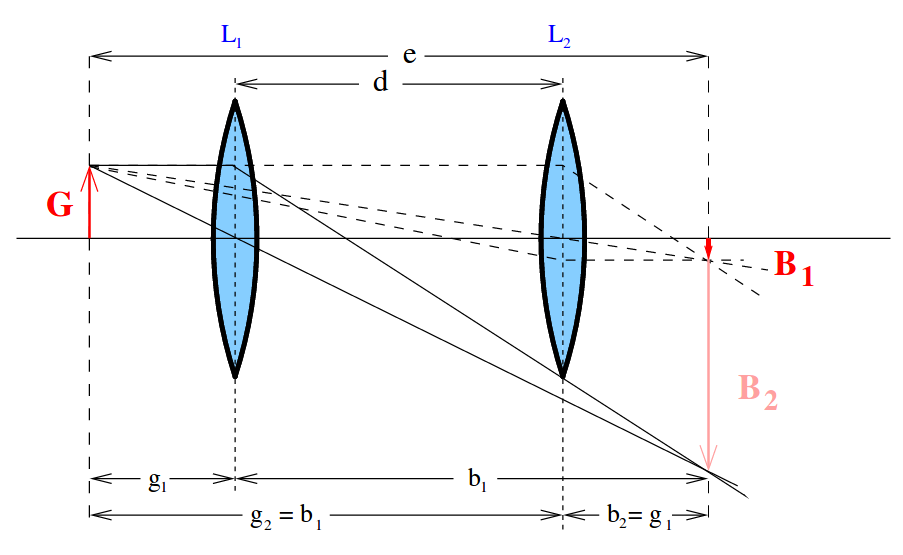
\includegraphics[width=0.8\textwidth]{V4082.png}
  \caption{Aufbau für die Methode von Bessel \cite{anleitung}.}
  \label{fig:V4082}
\end{figure}
\clearpage
\begin{figure}[htb]
  \centering
  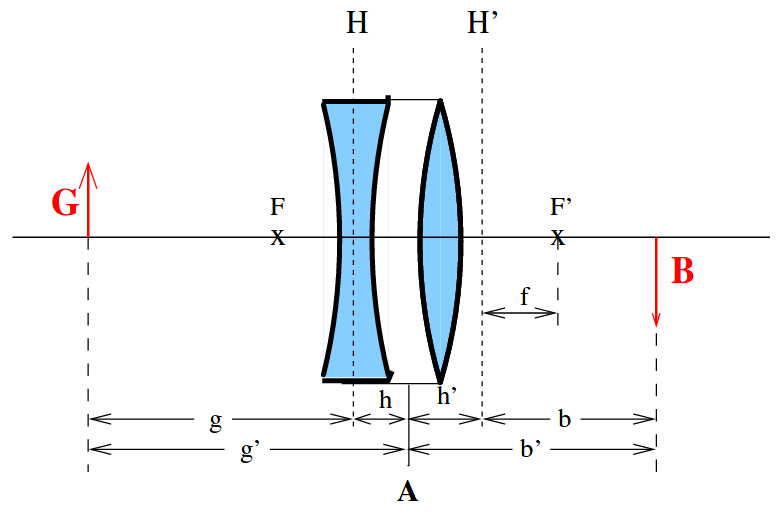
\includegraphics[width=0.8\textwidth]{V4083.png}
  \caption{Aufbau für die Methode von Abbe \cite{anleitung}.}
  \label{fig:V4083}
\end{figure}
\subsection{Versuchsablauf}
Der Versuch besteht aus drei Abschnitten.

\noindent
Zuerst sollen das Abbildungsgesetz und die Linsengleichung überprüft werden.
Hierzu wird eine Linse mit bekannter Brennweite (in unserem Fall \SI{100}{\milli\meter})
verwendet. Diese wird dann in zehn verschiedenen Abständen zum Gegenstand
platziert und entsprechend der Abstand des Schirms für eine scharfe Abbildung
angepasst. Dabei werden die Gegenstandsweite, die Bildweite und bei fünf
Messungen zusätzlich die Bildgröße notiert.
Danach wird die Messung für eine unbekannte Linse wiederholt. Jedoch ohne
dabei die Bildgröße zu notieren.

\noindent
Im zweiten Abschnitt soll die Brennweite einer Linse mit der Methode von
Bessel bestimmt werden. Hierzu wird der Schirm in einem festen Abstand
zum Gegenstand platziert. Aufgrund des festen Abstands gibt es dann zwei
Symmetriepunkte, in denen Bild- und Gegenstandsweite, bei scharfer
Abbildung, die jeweils zum anderen Symmetriepunkt vertauschten Werte
annehmen (wie in Abbildung \ref{fig:V4082} zu sehen). Die Gegenstands-
und Bildweite beider Punkte werden dann für zehn verschiedene Abstände
zwischen Gegenstand und Schirm bestimmt. Anschließend wird die gleiche
Messung jeweils fünf mal mit einem roten und einem blauen Filter vor
dem Gegenstand durchgeführt.

\noindent
Im letzten Abschnitt soll die Brennweite eines Linsensystems mit der Methode
von Abbe bestimmt werden. Hierzu werden zwei Linsen verwendet. Eine Linse
mit einer Brennweite von \SI{-100}{\milli\meter} und eine Linse mit einer
Brennweite von \SI{100}{\milli\meter}. Diese werden möglichst dicht beisammen,
in der Reihenfolge wie sie in Abbildung \ref{fig:V4083} zu sehen ist, zwischen
Gegenstand und Schirm platziert. Nun wird ein Referenzpunkt $A$ gewählt,
von welchem aus im Folgenden immer der Abstand zu Schirm und Gegenstand
bestimmt wird. Die Linsen werden nun in zehn verschiedene Positionen gebracht
und der Schirm für eine scharfe Abbildung verschoben.
Für jede Position der Linsen wird dann der Abstand zum Schirm, der Abstand zum
Gegenstand und der Abbildungsmaßstab (Bildgröße messen und nach \eqref{eqn:abbildung}
ausrechnen) bestimmt.

\end{document}
